\documentclass{standalone}
\usepackage{tikz}
\usetikzlibrary{patterns, positioning}

\begin{document}
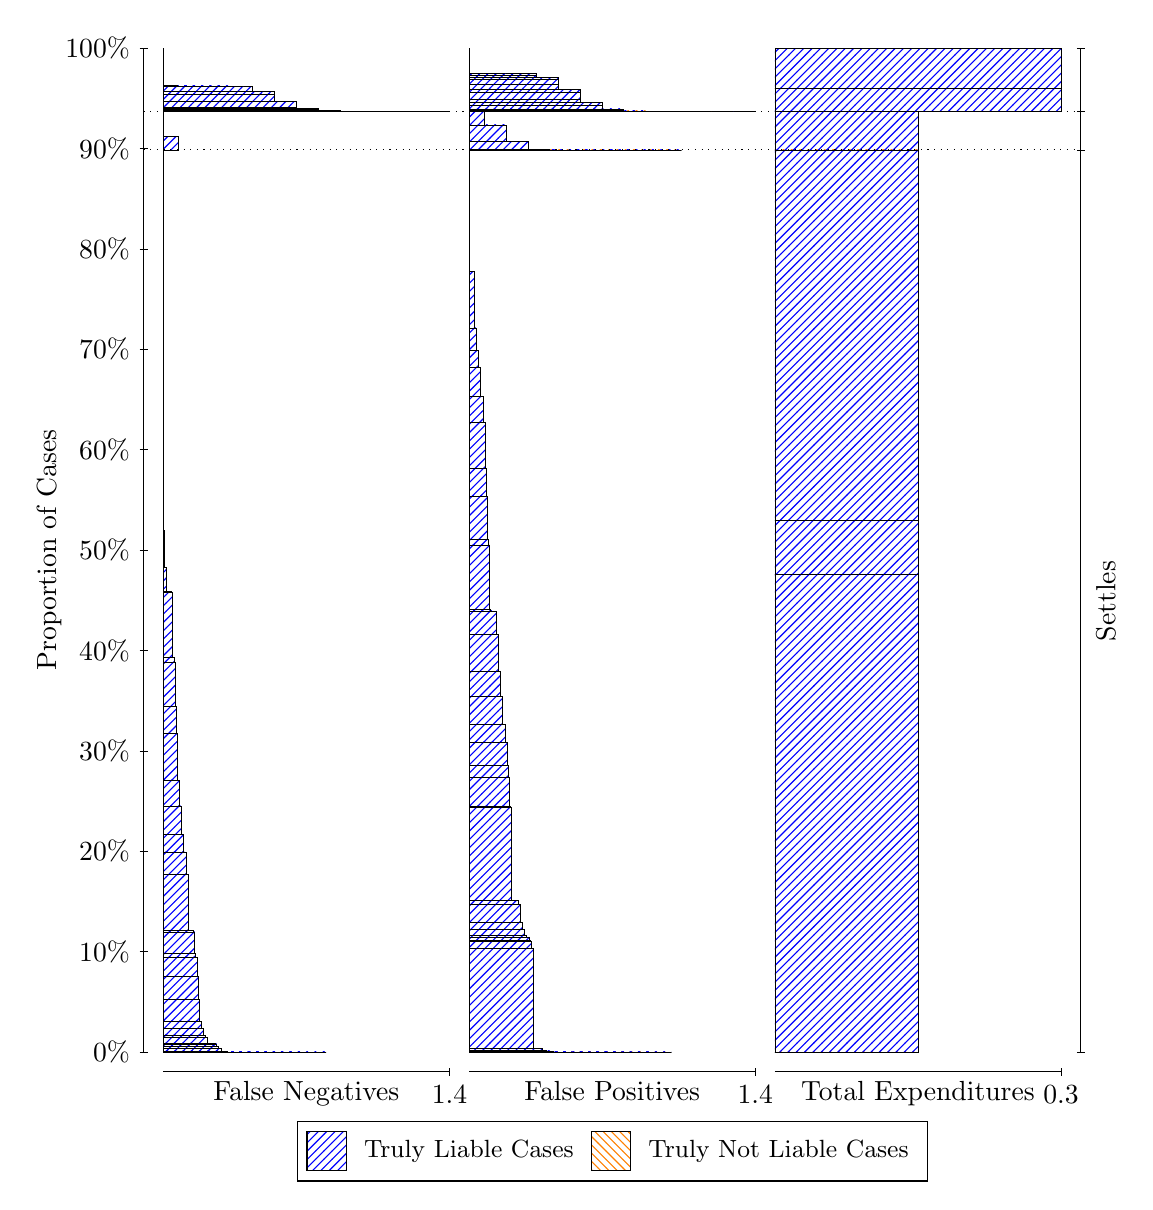
\begin{tikzpicture}
\draw[black, very thin] (1.5,1.75) -- (1.5,14.5);
\node[rotate=90, anchor=center] at (0.3, 8.125) {Proportion of Cases};
\draw[black, very thin] (1.45,1.75) -- (1.55,1.75);
\node[anchor=east] at (1.45, 1.75) {0\%};
\draw[black, very thin] (1.45,3.025) -- (1.55,3.025);
\node[anchor=east] at (1.45, 3.025) {10\%};
\draw[black, very thin] (1.45,4.3) -- (1.55,4.3);
\node[anchor=east] at (1.45, 4.3) {20\%};
\draw[black, very thin] (1.45,5.575) -- (1.55,5.575);
\node[anchor=east] at (1.45, 5.575) {30\%};
\draw[black, very thin] (1.45,6.85) -- (1.55,6.85);
\node[anchor=east] at (1.45, 6.85) {40\%};
\draw[black, very thin] (1.45,8.125) -- (1.55,8.125);
\node[anchor=east] at (1.45, 8.125) {50\%};
\draw[black, very thin] (1.45,9.4) -- (1.55,9.4);
\node[anchor=east] at (1.45, 9.4) {60\%};
\draw[black, very thin] (1.45,10.675) -- (1.55,10.675);
\node[anchor=east] at (1.45, 10.675) {70\%};
\draw[black, very thin] (1.45,11.95) -- (1.55,11.95);
\node[anchor=east] at (1.45, 11.95) {80\%};
\draw[black, very thin] (1.45,13.225) -- (1.55,13.225);
\node[anchor=east] at (1.45, 13.225) {90\%};
\draw[black, very thin] (1.45,14.5) -- (1.55,14.5);
\node[anchor=east] at (1.45, 14.5) {100\%};

\draw[black, very thin] (13.4,1.75) -- (13.4,14.5);
\draw[black, very thin] (13.35,1.75) -- (13.45,1.75);
\node[anchor=west] at (13.35, 1.75) {};
\draw[black, very thin] (13.35,13.206) -- (13.45,13.206);
\node[anchor=west] at (13.35, 13.206) {};
\draw[black, very thin] (13.35,13.699) -- (13.45,13.699);
\node[anchor=west] at (13.35, 13.699) {};
\draw[black, very thin] (13.35,14.5) -- (13.45,14.5);
\node[anchor=west] at (13.35, 14.5) {};

\draw[black, very thin, pattern color=blue, pattern=north east lines] (1.75,1.75) rectangle (3.8172,1.75);
\draw[black, very thin, pattern color=blue, pattern=north east lines] (1.75,1.75) rectangle (3.5667,1.75);
\draw[black, very thin, pattern color=blue, pattern=north east lines] (1.75,1.75) rectangle (3.5388,1.75);
\draw[black, very thin, pattern color=blue, pattern=north east lines] (1.75,1.75) rectangle (3.3161,1.75);
\draw[black, very thin, pattern color=blue, pattern=north east lines] (1.75,1.75) rectangle (3.2883,1.75);
\draw[black, very thin, pattern color=blue, pattern=north east lines] (1.75,1.75) rectangle (3.2604,1.75);
\draw[black, very thin, pattern color=blue, pattern=north east lines] (1.75,1.75) rectangle (3.0655,1.75);
\draw[black, very thin, pattern color=blue, pattern=north east lines] (1.75,1.75) rectangle (3.0377,1.75);
\draw[black, very thin, pattern color=blue, pattern=north east lines] (1.75,1.75) rectangle (3.0098,1.75);
\draw[black, very thin, pattern color=blue, pattern=north east lines] (1.75,1.75) rectangle (2.982,1.75);
\draw[black, very thin, pattern color=blue, pattern=north east lines] (1.75,1.75) rectangle (2.9402,1.75);
\draw[black, very thin, pattern color=blue, pattern=north east lines] (1.75,1.75) rectangle (2.8149,1.7501);
\draw[black, very thin, pattern color=blue, pattern=north east lines] (1.75,1.7501) rectangle (2.7871,1.7502);
\draw[black, very thin, pattern color=blue, pattern=north east lines] (1.75,1.7502) rectangle (2.7593,1.7507);
\draw[black, very thin, pattern color=blue, pattern=north east lines] (1.75,1.7507) rectangle (2.7314,1.7512);
\draw[black, very thin, pattern color=blue, pattern=north east lines] (1.75,1.7512) rectangle (2.7036,1.7518);
\draw[black, very thin, pattern color=blue, pattern=north east lines] (1.75,1.7518) rectangle (2.6897,1.7521);
\draw[black, very thin, pattern color=blue, pattern=north east lines] (1.75,1.7521) rectangle (2.6618,1.7521);
\draw[black, very thin, pattern color=blue, pattern=north east lines] (1.75,1.7521) rectangle (2.5644,1.7543);
\draw[black, very thin, pattern color=blue, pattern=north east lines] (1.75,1.7543) rectangle (2.5365,1.7587);
\draw[black, very thin, pattern color=blue, pattern=north east lines] (1.75,1.7587) rectangle (2.5087,1.7641);
\draw[black, very thin, pattern color=blue, pattern=north east lines] (1.75,1.7641) rectangle (2.4808,1.7917);
\draw[black, very thin, pattern color=blue, pattern=north east lines] (1.75,1.7917) rectangle (2.453,1.8174);
\draw[black, very thin, pattern color=blue, pattern=north east lines] (1.75,1.8174) rectangle (2.4391,1.8262);
\draw[black, very thin, pattern color=blue, pattern=north east lines] (1.75,1.8262) rectangle (2.4252,1.8525);
\draw[black, very thin, pattern color=blue, pattern=north east lines] (1.75,1.8525) rectangle (2.4112,1.8571);
\draw[black, very thin, pattern color=blue, pattern=north east lines] (1.75,1.8571) rectangle (2.3834,1.8572);
\draw[black, very thin, pattern color=blue, pattern=north east lines] (1.75,1.8572) rectangle (2.3138,1.9313);
\draw[black, very thin, pattern color=blue, pattern=north east lines] (1.75,1.9313) rectangle (2.286,1.9684);
\draw[black, very thin, pattern color=blue, pattern=north east lines] (1.75,1.9684) rectangle (2.2581,2.0473);
\draw[black, very thin, pattern color=blue, pattern=north east lines] (1.75,2.0473) rectangle (2.2303,2.1456);
\draw[black, very thin, pattern color=blue, pattern=north east lines] (1.75,2.1456) rectangle (2.2024,2.419);
\draw[black, very thin, pattern color=blue, pattern=north east lines] (1.75,2.419) rectangle (2.1885,2.7118);
\draw[black, very thin, pattern color=blue, pattern=north east lines] (1.75,2.7118) rectangle (2.1746,2.9575);
\draw[black, very thin, pattern color=blue, pattern=north east lines] (1.75,2.9575) rectangle (2.1607,3.0027);
\draw[black, very thin, pattern color=blue, pattern=north east lines] (1.75,3.0027) rectangle (2.1467,3.2745);
\draw[black, very thin, pattern color=blue, pattern=north east lines] (1.75,3.2745) rectangle (2.1328,3.2942);
\draw[black, very thin, pattern color=blue, pattern=north east lines] (1.75,3.2942) rectangle (2.105,3.2946);
\draw[black, very thin, pattern color=blue, pattern=north east lines] (1.75,3.2946) rectangle (2.0632,4.0097);
\draw[black, very thin, pattern color=blue, pattern=north east lines] (1.75,4.0097) rectangle (2.0354,4.292);
\draw[black, very thin, pattern color=blue, pattern=north east lines] (1.75,4.292) rectangle (2.0075,4.5097);
\draw[black, very thin, pattern color=blue, pattern=north east lines] (1.75,4.5097) rectangle (1.9797,4.8758);
\draw[black, very thin, pattern color=blue, pattern=north east lines] (1.75,4.8758) rectangle (1.9519,5.2067);
\draw[black, very thin, pattern color=blue, pattern=north east lines] (1.75,5.2067) rectangle (1.924,5.7992);
\draw[black, very thin, pattern color=blue, pattern=north east lines] (1.75,5.7992) rectangle (1.9101,6.1428);
\draw[black, very thin, pattern color=blue, pattern=north east lines] (1.75,6.1428) rectangle (1.8962,6.6935);
\draw[black, very thin, pattern color=blue, pattern=north east lines] (1.75,6.6935) rectangle (1.8822,6.7651);
\draw[black, very thin, pattern color=blue, pattern=north east lines] (1.75,6.7651) rectangle (1.8683,7.5851);
\draw[black, very thin, pattern color=blue, pattern=north east lines] (1.75,7.5851) rectangle (1.8544,7.6037);
\draw[black, very thin, pattern color=blue, pattern=north east lines] (1.75,7.6037) rectangle (1.8266,7.6041);
\draw[black, very thin, pattern color=blue, pattern=north east lines] (1.75,7.6041) rectangle (1.7848,7.9061);
\draw[black, very thin, pattern color=blue, pattern=north east lines] (1.75,7.9061) rectangle (1.757,8.3758);
\draw[black, very thin, pattern color=orange, pattern=north west lines] (1.75,8.3758) rectangle (1.75,8.3758);
\draw[black, very thin, pattern color=blue, pattern=north east lines] (1.75,8.3758) rectangle (1.75,13.206);
\draw[black, very thin, pattern color=blue, pattern=north east lines] (1.75,13.206) rectangle (1.9379,13.379);
\draw[black, very thin, pattern color=orange, pattern=north west lines] (1.75,13.379) rectangle (1.75,13.379);
\draw[black, very thin, pattern color=blue, pattern=north east lines] (1.75,13.379) rectangle (1.75,13.699);
\draw[black, very thin, pattern color=blue, pattern=north east lines] (1.75,13.699) rectangle (5.3833,13.699);
\draw[black, very thin, pattern color=blue, pattern=north east lines] (1.75,13.699) rectangle (5.1049,13.699);
\draw[black, very thin, pattern color=blue, pattern=north east lines] (1.75,13.699) rectangle (4.8265,13.699);
\draw[black, very thin, pattern color=blue, pattern=north east lines] (1.75,13.699) rectangle (4.8265,13.699);
\draw[black, very thin, pattern color=blue, pattern=north east lines] (1.75,13.699) rectangle (4.5481,13.699);
\draw[black, very thin, pattern color=blue, pattern=north east lines] (1.75,13.699) rectangle (4.2697,13.699);
\draw[black, very thin, pattern color=blue, pattern=north east lines] (1.75,13.699) rectangle (3.9913,13.705);
\draw[black, very thin, pattern color=blue, pattern=north east lines] (1.75,13.705) rectangle (3.7128,13.716);
\draw[black, very thin, pattern color=blue, pattern=north east lines] (1.75,13.716) rectangle (3.7128,13.733);
\draw[black, very thin, pattern color=blue, pattern=north east lines] (1.75,13.733) rectangle (3.4344,13.75);
\draw[black, very thin, pattern color=blue, pattern=north east lines] (1.75,13.75) rectangle (3.4344,13.821);
\draw[black, very thin, pattern color=blue, pattern=north east lines] (1.75,13.821) rectangle (3.156,13.918);
\draw[black, very thin, pattern color=blue, pattern=north east lines] (1.75,13.918) rectangle (3.156,13.951);
\draw[black, very thin, pattern color=blue, pattern=north east lines] (1.75,13.951) rectangle (3.0446,13.951);
\draw[black, very thin, pattern color=blue, pattern=north east lines] (1.75,13.951) rectangle (2.8776,14.012);
\draw[black, very thin, pattern color=blue, pattern=north east lines] (1.75,14.012) rectangle (2.7662,14.012);
\draw[black, very thin, pattern color=blue, pattern=north east lines] (1.75,14.012) rectangle (2.5992,14.012);
\draw[black, very thin, pattern color=blue, pattern=north east lines] (1.75,14.012) rectangle (2.5992,14.016);
\draw[black, very thin, pattern color=blue, pattern=north east lines] (1.75,14.016) rectangle (2.5992,14.019);
\draw[black, very thin, pattern color=blue, pattern=north east lines] (1.75,14.019) rectangle (2.4878,14.019);
\draw[black, very thin, pattern color=blue, pattern=north east lines] (1.75,14.019) rectangle (2.4878,14.019);
\draw[black, very thin, pattern color=blue, pattern=north east lines] (1.75,14.019) rectangle (2.3208,14.019);
\draw[black, very thin, pattern color=blue, pattern=north east lines] (1.75,14.019) rectangle (2.3208,14.019);
\draw[black, very thin, pattern color=blue, pattern=north east lines] (1.75,14.019) rectangle (2.2094,14.02);
\draw[black, very thin, pattern color=blue, pattern=north east lines] (1.75,14.02) rectangle (2.2094,14.02);
\draw[black, very thin, pattern color=blue, pattern=north east lines] (1.75,14.02) rectangle (2.0423,14.02);
\draw[black, very thin, pattern color=blue, pattern=north east lines] (1.75,14.02) rectangle (2.0423,14.02);
\draw[black, very thin, pattern color=blue, pattern=north east lines] (1.75,14.02) rectangle (1.931,14.02);
\draw[black, very thin, pattern color=blue, pattern=north east lines] (1.75,14.02) rectangle (1.931,14.022);
\draw[black, very thin, pattern color=blue, pattern=north east lines] (1.75,14.022) rectangle (1.7639,14.022);
\draw[black, very thin, pattern color=blue, pattern=north east lines] (1.75,14.022) rectangle (1.7639,14.022);
\draw[black, very thin, pattern color=orange, pattern=north west lines] (1.75,14.022) rectangle (1.75,14.022);
\draw[black, very thin, pattern color=blue, pattern=north east lines] (1.75,14.022) rectangle (1.75,14.5);
\draw[black, very thin, pattern color=orange, pattern=north west lines] (5.6333,1.75) rectangle (8.2017,1.75);
\draw[black, very thin, pattern color=blue, pattern=north east lines] (5.6333,1.75) rectangle (8.2017,1.75);
\draw[black, very thin, pattern color=orange, pattern=north west lines] (5.6333,1.75) rectangle (8.0764,1.75);
\draw[black, very thin, pattern color=blue, pattern=north east lines] (5.6333,1.75) rectangle (8.0764,1.75);
\draw[black, very thin, pattern color=orange, pattern=north west lines] (5.6333,1.75) rectangle (7.9511,1.75);
\draw[black, very thin, pattern color=blue, pattern=north east lines] (5.6333,1.75) rectangle (7.9511,1.75);
\draw[black, very thin, pattern color=blue, pattern=north east lines] (5.6333,1.75) rectangle (7.9233,1.75);
\draw[black, very thin, pattern color=orange, pattern=north west lines] (5.6333,1.75) rectangle (7.8259,1.75);
\draw[black, very thin, pattern color=blue, pattern=north east lines] (5.6333,1.75) rectangle (7.8259,1.75);
\draw[black, very thin, pattern color=blue, pattern=north east lines] (5.6333,1.75) rectangle (7.798,1.75);
\draw[black, very thin, pattern color=orange, pattern=north west lines] (5.6333,1.75) rectangle (7.7006,1.75);
\draw[black, very thin, pattern color=blue, pattern=north east lines] (5.6333,1.75) rectangle (7.7006,1.75);
\draw[black, very thin, pattern color=blue, pattern=north east lines] (5.6333,1.75) rectangle (7.6727,1.75);
\draw[black, very thin, pattern color=blue, pattern=north east lines] (5.6333,1.75) rectangle (7.6449,1.75);
\draw[black, very thin, pattern color=orange, pattern=north west lines] (5.6333,1.75) rectangle (7.5753,1.75);
\draw[black, very thin, pattern color=blue, pattern=north east lines] (5.6333,1.75) rectangle (7.5753,1.75);
\draw[black, very thin, pattern color=blue, pattern=north east lines] (5.6333,1.75) rectangle (7.5474,1.75);
\draw[black, very thin, pattern color=blue, pattern=north east lines] (5.6333,1.75) rectangle (7.5196,1.75);
\draw[black, very thin, pattern color=orange, pattern=north west lines] (5.6333,1.75) rectangle (7.45,1.75);
\draw[black, very thin, pattern color=blue, pattern=north east lines] (5.6333,1.75) rectangle (7.45,1.75);
\draw[black, very thin, pattern color=blue, pattern=north east lines] (5.6333,1.75) rectangle (7.4222,1.75);
\draw[black, very thin, pattern color=blue, pattern=north east lines] (5.6333,1.75) rectangle (7.3943,1.75);
\draw[black, very thin, pattern color=blue, pattern=north east lines] (5.6333,1.75) rectangle (7.3665,1.75);
\draw[black, very thin, pattern color=orange, pattern=north west lines] (5.6333,1.75) rectangle (7.3247,1.75);
\draw[black, very thin, pattern color=blue, pattern=north east lines] (5.6333,1.75) rectangle (7.3247,1.75);
\draw[black, very thin, pattern color=blue, pattern=north east lines] (5.6333,1.75) rectangle (7.2969,1.75);
\draw[black, very thin, pattern color=blue, pattern=north east lines] (5.6333,1.75) rectangle (7.269,1.75);
\draw[black, very thin, pattern color=blue, pattern=north east lines] (5.6333,1.75) rectangle (7.2412,1.75);
\draw[black, very thin, pattern color=orange, pattern=north west lines] (5.6333,1.75) rectangle (7.1994,1.75);
\draw[black, very thin, pattern color=blue, pattern=north east lines] (5.6333,1.75) rectangle (7.1994,1.75);
\draw[black, very thin, pattern color=blue, pattern=north east lines] (5.6333,1.75) rectangle (7.1716,1.75);
\draw[black, very thin, pattern color=blue, pattern=north east lines] (5.6333,1.75) rectangle (7.1437,1.75);
\draw[black, very thin, pattern color=blue, pattern=north east lines] (5.6333,1.75) rectangle (7.1159,1.75);
\draw[black, very thin, pattern color=blue, pattern=north east lines] (5.6333,1.75) rectangle (7.0881,1.75);
\draw[black, very thin, pattern color=blue, pattern=north east lines] (5.6333,1.75) rectangle (7.0463,1.75);
\draw[black, very thin, pattern color=blue, pattern=north east lines] (5.6333,1.75) rectangle (7.0185,1.75);
\draw[black, very thin, pattern color=blue, pattern=north east lines] (5.6333,1.75) rectangle (6.9906,1.75);
\draw[black, very thin, pattern color=blue, pattern=north east lines] (5.6333,1.75) rectangle (6.9628,1.75);
\draw[black, very thin, pattern color=orange, pattern=north west lines] (5.6333,1.75) rectangle (6.9489,1.75);
\draw[black, very thin, pattern color=blue, pattern=north east lines] (5.6333,1.75) rectangle (6.9489,1.75);
\draw[black, very thin, pattern color=blue, pattern=north east lines] (5.6333,1.75) rectangle (6.921,1.75);
\draw[black, very thin, pattern color=blue, pattern=north east lines] (5.6333,1.75) rectangle (6.8932,1.75);
\draw[black, very thin, pattern color=blue, pattern=north east lines] (5.6333,1.75) rectangle (6.8653,1.7501);
\draw[black, very thin, pattern color=blue, pattern=north east lines] (5.6333,1.7501) rectangle (6.8375,1.7506);
\draw[black, very thin, pattern color=blue, pattern=north east lines] (5.6333,1.7506) rectangle (6.8096,1.7506);
\draw[black, very thin, pattern color=blue, pattern=north east lines] (5.6333,1.7506) rectangle (6.7679,1.7506);
\draw[black, very thin, pattern color=blue, pattern=north east lines] (5.6333,1.7506) rectangle (6.74,1.7506);
\draw[black, very thin, pattern color=blue, pattern=north east lines] (5.6333,1.7506) rectangle (6.7122,1.7506);
\draw[black, very thin, pattern color=orange, pattern=north west lines] (5.6333,1.7506) rectangle (6.6983,1.7506);
\draw[black, very thin, pattern color=blue, pattern=north east lines] (5.6333,1.7506) rectangle (6.6983,1.7621);
\draw[black, very thin, pattern color=blue, pattern=north east lines] (5.6333,1.7621) rectangle (6.6844,1.7624);
\draw[black, very thin, pattern color=blue, pattern=north east lines] (5.6333,1.7624) rectangle (6.6704,1.7634);
\draw[black, very thin, pattern color=blue, pattern=north east lines] (5.6333,1.7634) rectangle (6.6426,1.7641);
\draw[black, very thin, pattern color=blue, pattern=north east lines] (5.6333,1.7641) rectangle (6.6148,1.767);
\draw[black, very thin, pattern color=blue, pattern=north east lines] (5.6333,1.767) rectangle (6.5869,1.7721);
\draw[black, very thin, pattern color=blue, pattern=north east lines] (5.6333,1.7721) rectangle (6.5591,1.797);
\draw[black, very thin, pattern color=blue, pattern=north east lines] (5.6333,1.797) rectangle (6.5312,1.7989);
\draw[black, very thin, pattern color=blue, pattern=north east lines] (5.6333,1.7989) rectangle (6.4895,1.7989);
\draw[black, very thin, pattern color=blue, pattern=north east lines] (5.6333,1.7989) rectangle (6.4616,1.7991);
\draw[black, very thin, pattern color=orange, pattern=north west lines] (5.6333,1.7991) rectangle (6.4477,1.7991);
\draw[black, very thin, pattern color=blue, pattern=north east lines] (5.6333,1.7991) rectangle (6.4477,3.0622);
\draw[black, very thin, pattern color=blue, pattern=north east lines] (5.6333,3.0622) rectangle (6.4338,3.0635);
\draw[black, very thin, pattern color=blue, pattern=north east lines] (5.6333,3.0635) rectangle (6.4199,3.1539);
\draw[black, very thin, pattern color=blue, pattern=north east lines] (5.6333,3.1539) rectangle (6.4059,3.1709);
\draw[black, very thin, pattern color=blue, pattern=north east lines] (5.6333,3.1709) rectangle (6.392,3.204);
\draw[black, very thin, pattern color=blue, pattern=north east lines] (5.6333,3.204) rectangle (6.3642,3.2329);
\draw[black, very thin, pattern color=blue, pattern=north east lines] (5.6333,3.2329) rectangle (6.3363,3.3046);
\draw[black, very thin, pattern color=blue, pattern=north east lines] (5.6333,3.3046) rectangle (6.3085,3.3984);
\draw[black, very thin, pattern color=blue, pattern=north east lines] (5.6333,3.3984) rectangle (6.2807,3.6251);
\draw[black, very thin, pattern color=blue, pattern=north east lines] (5.6333,3.6251) rectangle (6.2528,3.6736);
\draw[black, very thin, pattern color=blue, pattern=north east lines] (5.6333,3.6736) rectangle (6.211,3.6737);
\draw[black, very thin, pattern color=blue, pattern=north east lines] (5.6333,3.6737) rectangle (6.1832,3.6772);
\draw[black, very thin, pattern color=blue, pattern=north east lines] (5.6333,3.6772) rectangle (6.1693,4.853);
\draw[black, very thin, pattern color=blue, pattern=north east lines] (5.6333,4.853) rectangle (6.1554,4.8766);
\draw[black, very thin, pattern color=blue, pattern=north east lines] (5.6333,4.8766) rectangle (6.1414,5.2384);
\draw[black, very thin, pattern color=blue, pattern=north east lines] (5.6333,5.2384) rectangle (6.1275,5.3927);
\draw[black, very thin, pattern color=blue, pattern=north east lines] (5.6333,5.3927) rectangle (6.1136,5.687);
\draw[black, very thin, pattern color=blue, pattern=north east lines] (5.6333,5.687) rectangle (6.0858,5.9058);
\draw[black, very thin, pattern color=blue, pattern=north east lines] (5.6333,5.9058) rectangle (6.0579,6.266);
\draw[black, very thin, pattern color=blue, pattern=north east lines] (5.6333,6.266) rectangle (6.0301,6.5801);
\draw[black, very thin, pattern color=blue, pattern=north east lines] (5.6333,6.5801) rectangle (6.0022,7.0497);
\draw[black, very thin, pattern color=blue, pattern=north east lines] (5.6333,7.0497) rectangle (5.9744,7.3517);
\draw[black, very thin, pattern color=blue, pattern=north east lines] (5.6333,7.3517) rectangle (5.9326,7.3521);
\draw[black, very thin, pattern color=blue, pattern=north east lines] (5.6333,7.3521) rectangle (5.9048,7.3707);
\draw[black, very thin, pattern color=blue, pattern=north east lines] (5.6333,7.3707) rectangle (5.8909,8.1908);
\draw[black, very thin, pattern color=blue, pattern=north east lines] (5.6333,8.1908) rectangle (5.8769,8.2623);
\draw[black, very thin, pattern color=blue, pattern=north east lines] (5.6333,8.2623) rectangle (5.863,8.8131);
\draw[black, very thin, pattern color=blue, pattern=north east lines] (5.6333,8.8131) rectangle (5.8491,9.1566);
\draw[black, very thin, pattern color=blue, pattern=north east lines] (5.6333,9.1566) rectangle (5.8352,9.7492);
\draw[black, very thin, pattern color=blue, pattern=north east lines] (5.6333,9.7492) rectangle (5.8073,10.08);
\draw[black, very thin, pattern color=blue, pattern=north east lines] (5.6333,10.08) rectangle (5.7795,10.446);
\draw[black, very thin, pattern color=blue, pattern=north east lines] (5.6333,10.446) rectangle (5.7517,10.664);
\draw[black, very thin, pattern color=blue, pattern=north east lines] (5.6333,10.664) rectangle (5.7238,10.946);
\draw[black, very thin, pattern color=blue, pattern=north east lines] (5.6333,10.946) rectangle (5.696,11.661);
\draw[black, very thin, pattern color=blue, pattern=north east lines] (5.6333,11.661) rectangle (5.6542,11.662);
\draw[black, very thin, pattern color=blue, pattern=north east lines] (5.6333,11.662) rectangle (5.6333,13.206);
\draw[black, very thin, pattern color=orange, pattern=north west lines] (5.6333,13.206) rectangle (8.327,13.206);
\draw[black, very thin, pattern color=blue, pattern=north east lines] (5.6333,13.206) rectangle (8.327,13.206);
\draw[black, very thin, pattern color=blue, pattern=north east lines] (5.6333,13.206) rectangle (8.0486,13.206);
\draw[black, very thin, pattern color=blue, pattern=north east lines] (5.6333,13.206) rectangle (7.7702,13.206);
\draw[black, very thin, pattern color=blue, pattern=north east lines] (5.6333,13.206) rectangle (7.4918,13.206);
\draw[black, very thin, pattern color=blue, pattern=north east lines] (5.6333,13.206) rectangle (7.2133,13.206);
\draw[black, very thin, pattern color=blue, pattern=north east lines] (5.6333,13.206) rectangle (6.9349,13.206);
\draw[black, very thin, pattern color=blue, pattern=north east lines] (5.6333,13.206) rectangle (6.6565,13.217);
\draw[black, very thin, pattern color=blue, pattern=north east lines] (5.6333,13.217) rectangle (6.3781,13.313);
\draw[black, very thin, pattern color=blue, pattern=north east lines] (5.6333,13.313) rectangle (6.0997,13.525);
\draw[black, very thin, pattern color=blue, pattern=north east lines] (5.6333,13.525) rectangle (5.8213,13.699);
\draw[black, very thin, pattern color=orange, pattern=north west lines] (5.6333,13.699) rectangle (9.2667,13.699);
\draw[black, very thin, pattern color=blue, pattern=north east lines] (5.6333,13.699) rectangle (9.2667,13.699);
\draw[black, very thin, pattern color=orange, pattern=north west lines] (5.6333,13.699) rectangle (8.9883,13.699);
\draw[black, very thin, pattern color=blue, pattern=north east lines] (5.6333,13.699) rectangle (8.9883,13.699);
\draw[black, very thin, pattern color=orange, pattern=north west lines] (5.6333,13.699) rectangle (8.7098,13.699);
\draw[black, very thin, pattern color=blue, pattern=north east lines] (5.6333,13.699) rectangle (8.7098,13.699);
\draw[black, very thin, pattern color=blue, pattern=north east lines] (5.6333,13.699) rectangle (8.7098,13.699);
\draw[black, very thin, pattern color=orange, pattern=north west lines] (5.6333,13.699) rectangle (8.4314,13.699);
\draw[black, very thin, pattern color=blue, pattern=north east lines] (5.6333,13.699) rectangle (8.4314,13.699);
\draw[black, very thin, pattern color=orange, pattern=north west lines] (5.6333,13.699) rectangle (8.153,13.699);
\draw[black, very thin, pattern color=blue, pattern=north east lines] (5.6333,13.699) rectangle (8.153,13.699);
\draw[black, very thin, pattern color=blue, pattern=north east lines] (5.6333,13.699) rectangle (7.8746,13.7);
\draw[black, very thin, pattern color=blue, pattern=north east lines] (5.6333,13.7) rectangle (7.8746,13.701);
\draw[black, very thin, pattern color=orange, pattern=north west lines] (5.6333,13.701) rectangle (7.8746,13.701);
\draw[black, very thin, pattern color=blue, pattern=north east lines] (5.6333,13.701) rectangle (7.8746,13.703);
\draw[black, very thin, pattern color=blue, pattern=north east lines] (5.6333,13.703) rectangle (7.5962,13.712);
\draw[black, very thin, pattern color=blue, pattern=north east lines] (5.6333,13.712) rectangle (7.5962,13.721);
\draw[black, very thin, pattern color=orange, pattern=north west lines] (5.6333,13.721) rectangle (7.5962,13.721);
\draw[black, very thin, pattern color=blue, pattern=north east lines] (5.6333,13.721) rectangle (7.5962,13.728);
\draw[black, very thin, pattern color=blue, pattern=north east lines] (5.6333,13.728) rectangle (7.3178,13.772);
\draw[black, very thin, pattern color=blue, pattern=north east lines] (5.6333,13.772) rectangle (7.3178,13.811);
\draw[black, very thin, pattern color=blue, pattern=north east lines] (5.6333,13.811) rectangle (7.3178,13.812);
\draw[black, very thin, pattern color=orange, pattern=north west lines] (5.6333,13.812) rectangle (7.2064,13.812);
\draw[black, very thin, pattern color=blue, pattern=north east lines] (5.6333,13.812) rectangle (7.2064,13.812);
\draw[black, very thin, pattern color=blue, pattern=north east lines] (5.6333,13.812) rectangle (7.0393,13.845);
\draw[black, very thin, pattern color=blue, pattern=north east lines] (5.6333,13.845) rectangle (7.0393,13.939);
\draw[black, very thin, pattern color=blue, pattern=north east lines] (5.6333,13.939) rectangle (7.0393,13.977);
\draw[black, very thin, pattern color=orange, pattern=north west lines] (5.6333,13.977) rectangle (6.928,13.977);
\draw[black, very thin, pattern color=blue, pattern=north east lines] (5.6333,13.977) rectangle (6.928,13.977);
\draw[black, very thin, pattern color=blue, pattern=north east lines] (5.6333,13.977) rectangle (6.7609,14.034);
\draw[black, very thin, pattern color=blue, pattern=north east lines] (5.6333,14.034) rectangle (6.7609,14.099);
\draw[black, very thin, pattern color=blue, pattern=north east lines] (5.6333,14.099) rectangle (6.7609,14.131);
\draw[black, very thin, pattern color=orange, pattern=north west lines] (5.6333,14.131) rectangle (6.6496,14.131);
\draw[black, very thin, pattern color=blue, pattern=north east lines] (5.6333,14.131) rectangle (6.6496,14.131);
\draw[black, very thin, pattern color=blue, pattern=north east lines] (5.6333,14.131) rectangle (6.6496,14.131);
\draw[black, very thin, pattern color=blue, pattern=north east lines] (5.6333,14.131) rectangle (6.4825,14.133);
\draw[black, very thin, pattern color=blue, pattern=north east lines] (5.6333,14.133) rectangle (6.4825,14.159);
\draw[black, very thin, pattern color=blue, pattern=north east lines] (5.6333,14.159) rectangle (6.4825,14.176);
\draw[black, very thin, pattern color=blue, pattern=north east lines] (5.6333,14.176) rectangle (6.3711,14.176);
\draw[black, very thin, pattern color=orange, pattern=north west lines] (5.6333,14.176) rectangle (6.3711,14.176);
\draw[black, very thin, pattern color=blue, pattern=north east lines] (5.6333,14.176) rectangle (6.3711,14.176);
\draw[black, very thin, pattern color=blue, pattern=north east lines] (5.6333,14.176) rectangle (6.2041,14.177);
\draw[black, very thin, pattern color=blue, pattern=north east lines] (5.6333,14.177) rectangle (6.2041,14.178);
\draw[black, very thin, pattern color=blue, pattern=north east lines] (5.6333,14.178) rectangle (6.2041,14.179);
\draw[black, very thin, pattern color=blue, pattern=north east lines] (5.6333,14.179) rectangle (6.0927,14.179);
\draw[black, very thin, pattern color=orange, pattern=north west lines] (5.6333,14.179) rectangle (6.0927,14.179);
\draw[black, very thin, pattern color=blue, pattern=north east lines] (5.6333,14.179) rectangle (6.0927,14.179);
\draw[black, very thin, pattern color=blue, pattern=north east lines] (5.6333,14.179) rectangle (6.0927,14.179);
\draw[black, very thin, pattern color=blue, pattern=north east lines] (5.6333,14.179) rectangle (5.9257,14.179);
\draw[black, very thin, pattern color=blue, pattern=north east lines] (5.6333,14.179) rectangle (5.9257,14.179);
\draw[black, very thin, pattern color=blue, pattern=north east lines] (5.6333,14.179) rectangle (5.8143,14.179);
\draw[black, very thin, pattern color=orange, pattern=north west lines] (5.6333,14.179) rectangle (5.8143,14.179);
\draw[black, very thin, pattern color=blue, pattern=north east lines] (5.6333,14.179) rectangle (5.8143,14.179);
\draw[black, very thin, pattern color=blue, pattern=north east lines] (5.6333,14.179) rectangle (5.8143,14.179);
\draw[black, very thin, pattern color=blue, pattern=north east lines] (5.6333,14.179) rectangle (5.6473,14.179);
\draw[black, very thin, pattern color=blue, pattern=north east lines] (5.6333,14.179) rectangle (5.6473,14.179);
\draw[black, very thin, pattern color=orange, pattern=north west lines] (5.6333,14.179) rectangle (5.6333,14.179);
\draw[black, very thin, pattern color=blue, pattern=north east lines] (5.6333,14.179) rectangle (5.6333,14.5);
\draw[black, very thin, pattern color=orange, pattern=north west lines] (9.5167,1.75) rectangle (11.333,1.75);
\draw[black, very thin, pattern color=blue, pattern=north east lines] (9.5167,1.75) rectangle (11.333,7.8166);
\draw[black, very thin, pattern color=orange, pattern=north west lines] (9.5167,7.8166) rectangle (11.333,7.8166);
\draw[black, very thin, pattern color=blue, pattern=north east lines] (9.5167,7.8166) rectangle (11.333,8.4996);
\draw[black, very thin, pattern color=orange, pattern=north west lines] (9.5167,8.4996) rectangle (11.333,8.4996);
\draw[black, very thin, pattern color=blue, pattern=north east lines] (9.5167,8.4996) rectangle (11.333,13.206);
\draw[black, very thin, pattern color=orange, pattern=north west lines] (9.5167,13.206) rectangle (11.333,13.206);
\draw[black, very thin, pattern color=blue, pattern=north east lines] (9.5167,13.206) rectangle (11.333,13.699);
\draw[black, very thin, pattern color=orange, pattern=north west lines] (9.5167,13.699) rectangle (13.15,13.699);
\draw[black, very thin, pattern color=blue, pattern=north east lines] (9.5167,13.699) rectangle (13.15,13.983);
\draw[black, very thin, pattern color=orange, pattern=north west lines] (9.5167,13.983) rectangle (13.15,13.983);
\draw[black, very thin, pattern color=blue, pattern=north east lines] (9.5167,13.983) rectangle (13.15,14.5);
\draw[black, dotted] (1.5,13.206) -- (13.4,13.206);
\draw[black, dotted] (1.5,13.699) -- (13.4,13.699);
\draw[black, very thin] (1.75,1.5) -- (5.3833,1.5);
\node[anchor=north] at (3.5667, 1.5) {False Negatives};
\draw[black, very thin] (5.3833,1.45) -- (5.3833,1.55);
\node[anchor=north] at (5.3833, 1.45) {1.4};

\draw[black, very thin] (5.6333,1.5) -- (9.2667,1.5);
\node[anchor=north] at (7.45, 1.5) {False Positives};
\draw[black, very thin] (9.2667,1.45) -- (9.2667,1.55);
\node[anchor=north] at (9.2667, 1.45) {1.4};

\draw[black, very thin] (9.5167,1.5) -- (13.15,1.5);
\node[anchor=north] at (11.333, 1.5) {Total Expenditures};
\draw[black, very thin] (13.15,1.45) -- (13.15,1.55);
\node[anchor=north] at (13.15, 1.45) {0.3};

\node[black, centered, rotate=90] at (13.72, 7.4779) {Settles};



\draw (7.449999999999999,1.5) node[draw=none] (baseCoordinate) {};
\begin{scope}[align=center]
        \matrix[scale=0.5, draw=black, below=0.5cm of baseCoordinate, nodes={draw}, column sep=0.1cm]{
            \node[rectangle, draw, minimum width=0.5cm, minimum height=0.5cm, pattern=north east lines, pattern color=blue] {}; &
            \node[draw=none, font=\small] (B) {Truly Liable Cases}; &
            \node[rectangle, draw, minimum width=0.5cm, minimum height=0.5cm, pattern=north west lines, pattern color=orange] {}; &
            \node[draw=none, font=\small] (B) {Truly Not Liable Cases}; \\
            };
\end{scope}

\end{tikzpicture}
\end{document}